\documentclass{scrartcl}
\usepackage{url,hyperref}
\usepackage{listings}
\usepackage{color,float,caption}
\usepackage{graphicx} 
\usepackage{booktabs}
\usepackage{longtable}
 
\definecolor{codegreen}{rgb}{0,0.6,0}
\definecolor{codegray}{rgb}{0.5,0.5,0.5}
\definecolor{codepurple}{rgb}{0.58,0,0.82}
\definecolor{backcolour}{rgb}{0.95,0.95,0.92}
 
\lstdefinestyle{mystyle}{
    backgroundcolor=\color{backcolour},   
    commentstyle=\color{codegreen},
    keywordstyle=\color{magenta},
    numberstyle=\tiny\color{codegray},
    stringstyle=\color{codepurple},
    basicstyle=\small,
    breakatwhitespace=false,         
    breaklines=true,                 
    captionpos=b,                    
    keepspaces=true,                 
    numbers=left,                    
    numbersep=5pt,                  
    showspaces=false,                
    showstringspaces=false,
    showtabs=false,                  
    tabsize=2
}
 
\lstset{style=mystyle,basicstyle=\small\ttfamily}
\setkomafont{disposition}{\normalcolor\bfseries}
\renewcommand{\thesection}{\Roman{section}} 
\begin{document}

\title{Machine Learning Engineer Nanodegree}
\author{Ann-Kristin Juschka}
\subtitle{Capstone Project}
\maketitle

%\begin{abstract}
%The abstract text goes here.m
%\end{abstract}


\section{Definition}
%(approx. 1-2 pages)
%\begin{lstlisting}[language=Python]
%test
%\end{lstlisting}

\subsection*{Project Overview}
In this Nanodegree, \emph{Convolutional Neural Networks (CNNs)} are introduced that are most commonly used to analyze visual data.
In the deep learning project of the Nanodegree, we train CNNs to detect dogs in images and to classify dog breeds.
In general, object detection and classification is a classical task in machine learning. 

The aim of this project is to use CNNs to detect and classify brands in images with logos. For this, usually CNNs are trained with the dataset \emph{FlickrLogos-27} \cite{flickrlogos27} and \emph{FlickrLogos-32} \cite{flickrlogos32}; e.g. in \cite{BIANCO201723,DBLP:journals/corr/IandolaSGK15}. We are also interested in this task as we later wish to \emph{analyze sentiments} in twitter tweeds with pictures where a given company's logo is detected.
Due to time and size limits, we focus in this project on \emph{logo detection and classification}.
%In this section, look to provide a high-level overview of the project in layman’s terms. Questions to ask yourself when writing this section:
%
%Has an overview of the project been provided, such as the problem domain, project origin, and related datasets or input data?
%Has enough background information been given so that an uninformed reader would understand the problem domain and following problem statement?
\subsection*{Problem Statement}
While most logo datasets like \emph{FlickrLogos-27} \cite{flickrlogos27} and \emph{FlickrLogos-32} \cite{flickrlogos32} contain raw original logo graphics, we want to train our CNN on the in-the-wild logo dataset \emph{Logos in the Wild} \cite{logosinthewild} whose images contain logos as natural part. As this dataset includes in total 11,054 images with 32,850 annotated logo bounding boxes of 871 brands, it should be possible to train a CNN that achieves a high  accuracy or mean average precision (map).
This is a challenging task as the regions containg logos are small.


The main goal of this project is to use CNNs to \emph{classify the brand and company logos} from the Logos in the Wild dataset with high accuracy and mean average precision (map).
For this, we first train an own CNN architecture as done in the dog breeds project of the Nanodegree.
% with a convolutionary layer, a max-pooling layer, another convolutionary layer, a max-pooling layer, a global-average pooling layer and a final fully connected layer.
Furthermore, to improve loss and accuracy we make use of the standard CNN architectures \emph{VGG19, Resnet50, InceptionV3, or Xception} that are already trained on the \emph{ImageNet} database \cite{kerasapplications}.
Moreover, as the dataset comes with annotations in Pascal-VOC style, if time permits we will also train a \emph{Faster Region-based Convolutional Neural Network (Faster R-CNN)} \cite{DBLP:journals/corr/RenHG015} for two stages: First, an \emph{Region Proposal Network (RPN)} for \emph{logo detection}, and second, a classifier like VGG19 for logo classification of the candidate regions.
 This Faster R-CNN will be evaluated using the \emph{mean average precision (map)} metric.
%In this section, you will want to clearly define the problem that you are trying to solve, including the strategy (outline of tasks) you will use to achieve the desired solution. You should also thoroughly discuss what the intended solution will be for this problem. Questions to ask yourself when writing this section:
%
%Is the problem statement clearly defined? Will the reader understand what you are expecting to solve?
%Have you thoroughly discussed how you will attempt to solve the problem?
%Is an anticipated solution clearly defined? Will the reader understand what results you are looking for?
\subsection*{Metrics}
For purely logo classification, we seek to achieve a high accuracy. \emph{Accuracy} is simply the number of correct predictions divided by the total number of predictions.

For logo detection, we need a different metric: \emph{mean average precision (map)} that is the mean over all classes, of the interpolated
\emph{average precision} \cite{everingham2010pascal} for each class. Recall that
\[
\textup{precision}=\frac{\textup{true positives}}{\textup{true positives}+\textup{false positives}},\quad \textup{recall}=\frac{\textup{true positives}}{\textup{true positives}+\textup{false negatives}}.
\]
Considering the precision-recall curve for a given threshold, and the interpolated precision $\textup{precision}_\textup{interpolated}(\textup{recall}_i)=\max_{\tilde{r},\tilde{r}\geq \textup{recall}_i}\textup{precision}(\tilde{r})$ of the 11 values $\textup{recall}_i=\{0,0.1,0.2,\ldots,0.9,1.0\}$. Then
\[
\textup{average precision}=\frac{1}{11}\sum_{1}^{11}\textup{precision}_\textup{interpolated}(\textup{recall}_i)\qquad\cite[\S\,4.2]{everingham2010pascal}.
\]
%In this section, you will need to clearly define the metrics or calculations you will use to measure performance of a model or result in your project. These calculations and metrics should be justified based on the characteristics of the problem and problem domain. Questions to ask yourself when writing this section:
%
%Are the metrics you’ve chosen to measure the performance of your models clearly discussed and defined?
%Have you provided reasonable justification for the metrics chosen based on the problem and solution?
\section{Analysis}
%(approx. 2-4 pages)

\subsection*{Data Exploration}
To train our model, we want to use the recent logo dataset \emph{Logos in the Wild} \cite{logosinthewild}. As mentioned above, the lastest version of this dataset (v2.0) contains 11,054 images with 32,850 annotated logo bounding boxes of 871 brands and it is collected by performing Google image searches with well-known brand and company names directly or in combination with a predefined set of search terms like ‘advertisement’, ‘building’, ‘poster’ or ‘store’.
The logo annotations are in Pascal-VOC style.

As stated by the creators of the Logo in the Wild dataset, this dataset has 4 to 608 images per searched brand, 
238 of 871 brands occur at least 10 times, and there are up to 118 logos in one image. Unfortunately, the dataset provides only the links to the images, and some of these images already disappeared.
As we later want to detect logos in arbitrary pictures from twitter tweeds, this large in-the-wild logo dataset still fits best to our goal. 

Instead of downloading ourselves the images from the different urls provided in the Logos in the Wild dataset, we download the \emph{QMUL-OpenLogo Dataset} \cite{DBLP:journals/corr/abs-1807-01964}, which contains Logos in the Wild as a subset including all available JPEG files.

We run a simple Python script to analyze the downloaded JPEG images in the Logos in the Wild dataset, and we find that in fact there are in total 821 brands, where the maximal number of logos per given brand is 1,928 for Heineken, and the minimum number is 1. Moreover, the image heineken/img00042.jpg contains the maximum of 118 logos, while in general every image contains at least one logo.
%
%In this section, you will be expected to analyze the data you are using for the problem. This data can either be in the form of a dataset (or datasets), input data (or input files), or even an environment. The type of data should be thoroughly described and, if possible, have basic statistics and information presented (such as discussion of input features or defining characteristics about the input or environment). Any abnormalities or interesting qualities about the data that may need to be addressed have been identified (such as features that need to be transformed or the possibility of outliers). Questions to ask yourself when writing this section:
%
%If a dataset is present for this problem, have you thoroughly discussed certain features about the dataset? Has a data sample been provided to the reader?
%If a dataset is present for this problem, are statistics about the dataset calculated and reported? Have any relevant results from this calculation been discussed?
%If a dataset is not present for this problem, has discussion been made about the input space or input data for your problem?
%Are there any abnormalities or characteristics about the input space or dataset that need to be addressed? (categorical variables, missing values, outliers, etc.)
%
\subsection*{Exploratory Visualization}
\begin{figure}[h!]
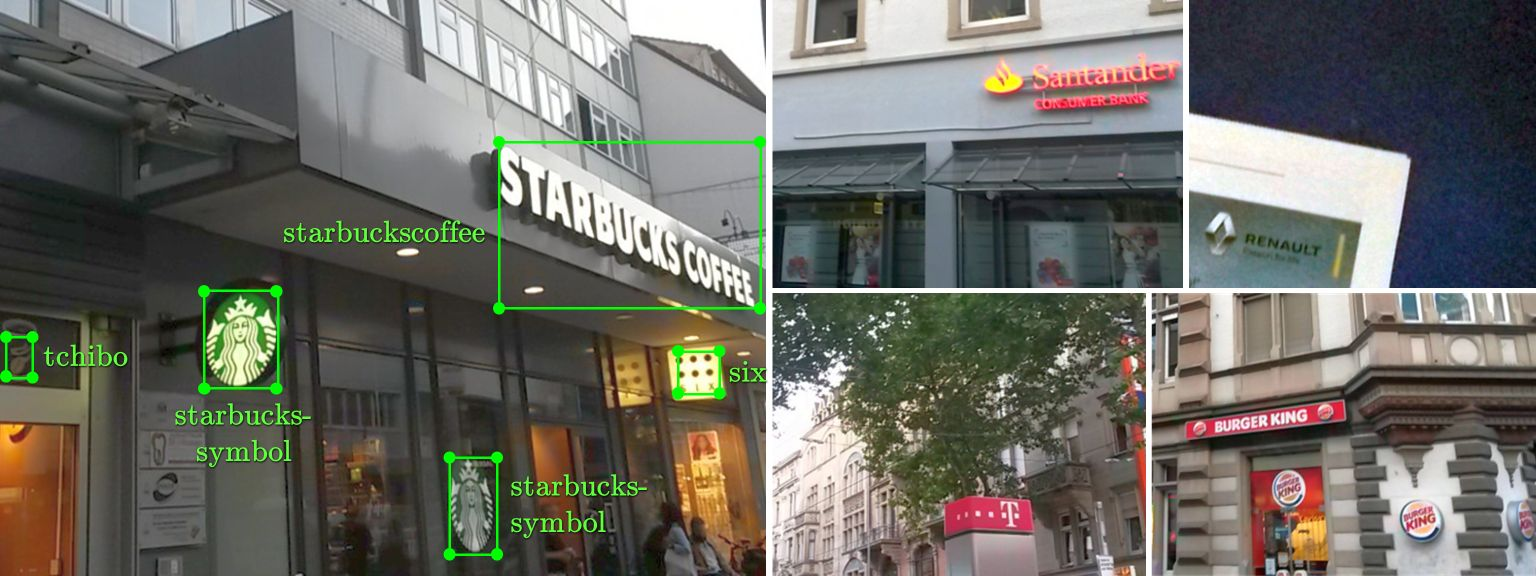
\includegraphics[width=\textwidth]{samples.jpg}
\caption[Bildbeschreibung]{\url{https://www.iosb.fraunhofer.de/servlet/is/78045/}}
\label{sampleImage}
\end{figure}
%\vspace*{-3em}%\captionof{figure}{\url{https://www.iosb.fraunhofer.de/servlet/is/78045/}}

While the images on the right contain logos of a single brand, the image on the left shows a sample image that includes bounding boxed for logos of different brands. In particular, an image can contain different types of logos of a brand. The following are the annotations in the Pascal-VOC style in the XML file corresponding to the image on the left hand side:

\begin{minipage}{.45\textwidth}
%<object>
%  <name>six</name>
%  <pose>Unspecified</pose>
%  <truncated>0</truncated>
%  <difficult>0</difficult>
%  <bndbox>
%    <xmin>633</xmin>
%    <ymin>327</ymin>
%    <xmax>671</xmax>
%    <ymax>365</ymax>
%  </bndbox>
%</object>
\begin{lstlisting}[basicstyle=\fontsize{7.5}{8}\ttfamily,language=xml]
<annotation>
  <folder>0samples</folder>
  <filename>img000009</filename>
  <path>\0samples\img000009.jpg</path>
  <source>
    <database>Unknown</database>
  </source>
  <size>
    <width>718</width>
    <height>535</height>
    <depth>3</depth>
  </size>
  <segmented>0</segmented>
  <object>
    <name>starbuckscoffee</name>
    <pose>Unspecified</pose>
    <truncated>0</truncated>
    <difficult>0</difficult>
    <bndbox>
      <xmin>466</xmin>
      <ymin>133</ymin>
      <xmax>709</xmax>
      <ymax>287</ymax>
    </bndbox>
  </object>
  <object>
    <name>starbucks-symbol</name>
    <pose>Unspecified</pose>
    <truncated>0</truncated>
    <difficult>0</difficult>
    <bndbox>
      <xmin>193</xmin>
      <ymin>270</ymin>
      <xmax>261</xmax>
      <ymax>360</ymax>
    </bndbox>
  </object>
\end{lstlisting}
\end{minipage}\hfill
\noindent\begin{minipage}{.45\textwidth}
%<object>
%  <name>tchibo</name>
%  <pose>Unspecified</pose>
%  <truncated>0</truncated>
%  <difficult>0</difficult>
%  <bndbox>
%    <xmin>8</xmin>
%    <ymin>312</ymin>
%    <xmax>34</xmax>
%    <ymax>351</ymax>
%  </bndbox>
%</object>
\begin{lstlisting}[basicstyle=\fontsize{7.5}{8}\ttfamily,language=xml,firstnumber=38]
  <object>
    <name>starbucks-symbol</name>
    <pose>Unspecified</pose>
    <truncated>0</truncated>
    <difficult>0</difficult>
    <bndbox>
      <xmin>420</xmin>
      <ymin>423</ymin>
      <xmax>464</xmax>
      <ymax>513</ymax>
    </bndbox>
  </object>
  <object>
    <name>six</name>
    <pose>Unspecified</pose>
    <truncated>0</truncated>
    <difficult>0</difficult>
    <bndbox>
      <xmin>633</xmin>
      <ymin>327</ymin>
      <xmax>671</xmax>
      <ymax>365</ymax>
    </bndbox>
  </object>
  <object>
    <name>tchibo</name>
    <pose>Unspecified</pose>
    <truncated>0</truncated>
    <difficult>0</difficult>
    <bndbox>
      <xmin>8</xmin>
      <ymin>312</ymin>
      <xmax>34</xmax>
      <ymax>351</ymax>
    </bndbox>
  </object>
</annotation>
\end{lstlisting}
\end{minipage}
%
%In this section, you will need to provide some form of visualization that summarizes or extracts a relevant characteristic or feature about the data. The visualization should adequately support the data being used. Discuss why this visualization was chosen and how it is relevant. Questions to ask yourself when writing this section:
%
%Have you visualized a relevant characteristic or feature about the dataset or input data?
%Is the visualization thoroughly analyzed and discussed?
%If a plot is provided, are the axes, title, and datum clearly defined?
\subsection*{Algorithms and Techniques}
%Probably we augment the training data to have more images per brand. 
As mentioned before, we start by training an own CNN architecture to classify the logos as done in the dog breeds project of the Nanodegree. For this, 40\% of the dataset forms the test set, and the remaining data is split into 80\% training set and 20\% validation set. Using Keras preprocessing, each image is converted into a 4D tensor with shape $(1,224,224,3)$.
This CNN consists of a convolutionary layer, a max-pooling layer, another convolutionary layer, a max-pooling layer, a global-average pooling layer and a final fully connected layer. 

The theory behind selecting these layer is that at first nodes in \emph{convolutionary layers} help to detect patterns in single small regions in the image by "filtering" images that are interpreted as 3D arrays (height, width and color).
In order to reduce overfitting caused by the high-dimensionality of the filter stack in the convolutionary layers we further use the following two types of \emph{pooling layers}:
Nodes in the first type \emph{max-pooling layer} contain the maximum value of the corresponding region in the filter stack of the previous layer. 
\emph{Global average pooling layers} reduce dimensionality more drastically by taking the average of the entries of each of the three 2D arrays, which constitute the image as 3D array, to produce a 3D vector. 

As gradient descent optimizer algorithm we choose "RMSprop", as loss function for our categorization problem "categorical cross entropy" and as metric "accuracy".
Using Keras ModelCheckpoint, we save the model with the best validation loss.

As a next step we train a popular CNN like VGG19 whose weights are pre-trained on ImageNet. We proceed similarly as in the first setting.

Having tried CNNs for logo classification, we finally proceed to Faster R-CNNs for logo detection and classification.
We first train a \emph{Region Proposal Network (RPN)} that proposes regions with logos in images.  The predicted region proposals are then reshaped using a \emph{Region of Interest (RoI)} pooling layer. This layer is next used to classify the image within the proposed region and predict the offset values for the bounding boxes. For the latter task, we again train a CNN like VGG19 that is pre-trained on ImageNet.
As  explained above, here we use mean average precision as metric.
%
%In this section, you will need to discuss the algorithms and techniques you intend to use for solving the problem. You should justify the use of each one based on the characteristics of the problem and the problem domain. Questions to ask yourself when writing this section:
%
%TODO
%Are the algorithms you will use, including any default variables/parameters in the project clearly defined?
%Are the techniques to be used thoroughly discussed and justified?
%Is it made clear how the input data or datasets will be handled by the algorithms and techniques chosen?

\subsection*{Benchmark}
The recent \emph{Logos in the Wild} dataset has not been studied much yet. When introduced in \cite{logosinthewild}, the focus is put on open set logo retrieval where only one sample image of a logo is available. 

Instead we want to focus on a closed world assumption where we train and test on the Logos in the Wild dataset which has multiple images per brand. 
Therefore, we can only compare our results with the ones of other models that were trained and tested on the popular closed dataset \emph{FlickrLogos-32} \cite{flickrlogos32}. As cited in \cite{logosinthewild}, the mean average precision (map) in state-of-the-art results is 0.811 achieved by Faster-RCNN \cite{DBLP:journals/corr/SuZG16}  where the training set is expanded with synthetically generated training images, and 0.842 using
Fast-M \cite{Bao:2016:RCL:3007669.3007728} that is a multi-scale Fast R-CNN based-approach.
%
%In this section, you will need to provide a clearly defined benchmark result or threshold for comparing across performances obtained by your solution. The reasoning behind the benchmark (in the case where it is not an established result) should be discussed. Questions to ask yourself when writing this section:
%
%Has some result or value been provided that acts as a benchmark for measuring performance?
%Is it clear how this result or value was obtained (whether by data or by hypothesis)?
\section{Methodology}
%(approx. 3-5 pages)

\subsection*{Data Preprocessing}
\label{dataPreprocessing}
Having gained access, we download the Logos in the Wild dataset \cite{logosinthewild} that contains XML files with the bounding boxes, the URLs to the JPEG images, samples and a script to obtain a clean dataset.
As stated above, we obtain the JPEG images of the Logos in the Wild dataset by downloading the superset QMUL-OpenLogo Dataset \cite{DBLP:journals/corr/abs-1807-01964}. 

After setting the variable "oldpath" to the absolute path of our \path{LogosInTheWild-v2/data} directory and the variable "new path" to the absolute path of our \path{openlogo/JPEGImages} directoy in our script move\_JPEG\_images.sh from the Logo Capstone Project, we execute this script that moves the JPEG files from the \path{openlogo/JPEGImages} directory in the corresponding brand subdirectory in the \path{LogosInTheWild-v2/data} directory.

Next we remove the \path{0samples} folder from the \path{LogosInTheWild-v2/data} directory, and execute in a separate Conda environment with Python 2.7 and opencv-python%the Python script \path{create\_clean\_dataset.py} from the \path{LogosInTheWild-v2/scripts} directory 
\begin{lstlisting}[language=bash]
# From LogosInTheWild-v2/scripts directory
python create_clean_dataset.py --roi --in ../data --out ../cleaned-data
\end{lstlisting}
that adjusts the brand names in the XML files and removes XML files without corresponding JPEG image.
This outputs that 9,428 images and 821 brands were processed, while 1,330 JPEG files were unavailable. In addition, it created 28,007 ROI images in corresponding folders with logo names.


For our first logo classification task with a standard CNN architecture in Keras and Python 3.6, we can load the image files with the \path{load_files} function from \path{sklearn.datasets} since the Logos in the Wild dataset is organized in directories with corresponding brand names. Of course, some images like the example in \autoref{sampleImage} contain logos of different brands so labelling them with the brand directory name may decrease accuracy.  Furthermore, we use the \path{image.load_img} and \path{image.img_to_array} functions from \path{keras.preprocessing} to convert the JPEG files to Keras' required 4D tensor format with shape $(1,224,224,3)$. As last preprocessing step for the first standard CNN architecture, we rescale the images by dividing every pixel in each image by 255.


Finally, for training a Faster R-CNN with Tensorflow's Object Detection API we need to convert the Logos in the Wild dataset with annotations in Pascal-VOC style to Tensorflow's TFRecord file format. For this, we copy the Python script \path{create_and_analyze_pascal_tf_record.py} from the Capstone project folder to the LogosInTheWild-v2 directory, rename the folder \path{LogosInTheWild-v2/cleaned_data} to \path{LogosInTheWild-v2/data}, enter "export PYTHONPATH=\$PYTHONPATH:`pwd`:`pwd`/slim
" when in the \path{tensorflow/models/research} directory and run the following:
%
%In this section, all of your preprocessing steps will need to be clearly documented, if any were necessary. From the previous section, any of the abnormalities or characteristics that you identified about the dataset will be addressed and corrected here. Questions to ask yourself when writing this section:


%If the algorithms chosen require preprocessing steps like feature selection or feature transformations, have they been properly documented?
%Based on the Data Exploration section, if there were abnormalities or characteristics that needed to be addressed, have they been properly corrected?
%If no preprocessing is needed, has it been made clear why?
\begin{lstlisting}[language=bash]
# From LogosInTheWild-v2 directory
python create_and_analyze_pascal_tf_record.py --data_dir=./data/voc_format --label_map_path=./data/pascal_label_map.pbtxt --output_path=./data/
\end{lstlisting}
%
%(py2) python object_detection/dataset_tools/create_pascal_tf_record.py --data_dir=/mnt/c/environment/Machine_Learning/Machine_Learning_Engineer/capstone_project/LogosInTheWild-v2/data/voc_format --year=VOC2012  --label_map_path=/mnt/c/environment/Machine_Learning/Machine_Learning_Engineer/capstone_project/LogosInTheWild-v2/data/pascal_label_map.pbtxt --output_path=/mnt/c/environment/Machine_Learning/Machine_Learning_Engineer/
%\begin{lstlisting}[language=bash]
%# From LogosInTheWild-v2 directory
%python analyze_pascal_tf_record.py --data_dir=./data/voc_format --year=VOC2012  --label_map_path=./data/pascal_label_map.pbtxt --output_path=./data/
%%
%%(py2) cd /mnt/c/ProgramData/anaconda3/envs/tensorflow/models/research
%%python object_detection/dataset_tools/analyze_pascal_tf_record.py --data_dir=/mnt/c/environment/Machine_Learning/Machine_Learning_Engineer/capstone_project/LogosInTheWild-v2/data/voc_format --year=VOC2012  --label_map_path=/mnt/c/environment/Machine_Learning/Machine_Learning_Engineer/capstone_project/LogosInTheWild-v2/data/pascal_label_map.pbtxt --output_path=/mnt/c/environment/Machine_Learning/Machine_Learning_Engineer/
%\end{lstlisting}
%TODO Modify create to analyze and remove 2 in pascal
After completion we see that we converted 6,034 images with annotations into the 10 training TFRecord files \path{pascal_train.record-0000i-of-00010}, and 1,508 images with annotations into the 10 validation TFRecord files \path{pascal_val.record-0000i-of-00010} for $i=0,\ldots,9$.
Further, in \path{LogosInTheWild-v2/data} this created \path{test_images.txt} containing the absolute path of the 1,886 images in the test set, and \path{pascal_label_map.pbtxt} containing 821 entries like the following:
\begin{lstlisting}[language=Python]
item {
  id: 262
  name: 'starbucks-text'
}
\end{lstlisting}
Among other parameters for our Faster R-CNN, we choose in our pipeline configuration file \path{faster_rcnn_inception_logos-locally-on-ubuntu.config} by the Capstone Project as data\_augmentation\_options random\_horizontal\_flip, random\_vertical\_flip and random\_rotation90.
    
\subsection*{Implementation}
\subsubsection*{A first CNN model from scratch in Keras \cite{chollet2015keras}}
For the logo classification task, we start to implement a standard Keras CNN architecture in the Jupyter notebook \path{logos.ipynb} located in the Capstone Project repository. Keras' model summary is as follows:
%\begin{table}[htb!]
%\centering
%\caption{Architecture of VGG-like CNN from Keras\cite{chollet2015keras}.}
%		\begin{tabular}{ccc}
%		\toprule
%		Layer (type) & Output Shape & Param \# \\
%		\midrule
%		conv2d\_1 (Conv2D) & (None, 14, 14, 32) & 320\\
%		conv2d\_2 (Conv2D) & (None, 12, 12, 32) & 9248\\
%		max\_pooling2d\_1 (MaxPooling2) & (None, 6, 6, 32) & 0\\
%		dropout\_1 (Dropout) & (None, 6, 6, 32) & 0\\
%		conv2d\_3 (Conv2D) & (None, 4, 4, 64) & 18496\\
%		conv2d\_4 (Conv2D) & (None, 2, 2, 64) & 36928\\
%		max\_pooling2d\_2 (MaxPooling2) & (None, 1, 1, 64) & 0\\
%		dropout\_2 (Dropout) & (None, 1, 1, 64) & 0\\
%		flatten\_1 (Flatten) & (None, 64) & 0\\
%		dense\_1 (Dense) & (None, 256) & 16640\\
%		dropout\_3 (Dropout) & (None, 256) & 0\\
%		dense\_2 (Dense) & (None, 10) & 2570\\
%		\bottomrule
%		\end{tabular}\\
%		\label{table:vgg}
%\end{table}
%
\begin{longtable}{ccc}%[htb!]
%\centering
\caption{Architecture of a first CNN for logo classification from Keras.}\\
    \hline
    Layer (type) & Output Shape & Param \# \\
    \hline
    \endfirsthead
    \multicolumn{3}{c}
    {\tablename\ \thetable\ -- \textit{Continued from previous page}} \\
%		\toprule
%\hline
%    Layer (type) & Output Shape & Param \# \\
%    \hline
\endhead
%    \hline 
    \multicolumn{3}{r}{\textit{Continued on next page}} \\
    \endfoot
%		\midrule
\hline\endlastfoot
conv2d\_3 (Conv2D)              &     (None, 223, 223, 32)    &   416       \\
max\_pooling2d\_4 (MaxPooling2) &     (None, 111, 111, 32)    &    0        \\
conv2d\_4 (Conv2D)              &     (None, 110, 110, 64)    &   8256      \\
max\_pooling2d\_5 (MaxPooling2) &     (None, 55, 55, 64)      &    0        \\
global\_average\_pooling2d\_2 (GAP2D\footnotemark)& (None, 64)&    0        \\ 
dense\_2 (Dense)                &     (None, 109)             &  7085       %\\
%		\bottomrule
%		\end{multicolumn}\\
		\label{table:modelFromScratch}
\end{longtable}
\footnotetext{GlobalAveragePooling2D}

This model has in total 15,757 parameters that are all trainable. We compile the model with optimizer 'rmsprop' and loss 'categorical\_crossentropy', and choose as  metric 'accuracy'. For training, we set epochs to 100, validation\_split to 0.3 and define a \path{ModelCheckpoint} from \path{keras.callbacks} that saves the model with the best validation loss.

After training and loading the model with the best weights, we compute the accuracy on the test images:
\begin{lstlisting}[language=Python]
print('\n', 'Test accuracy of the model from scratch:', model_from_scratch.evaluate(test_tensors, test_targets, verbose=0)[1]*100,'%.')
\end{lstlisting}
After training for 20 epochs, this results in "Test accuracy of the model from scratch: 16.76 \%". Finally, continuing to train for 600 further epochs leads to a test accuracy of 33.99 \% where the validation loss improved for the last time in epoch 594 to 2.95990. 

In the next section, we describe how we fine-tune our first model. 
\subsubsection*{A Custom Model on top of the VGG16 model \cite{DBLP:journals/corr/SimonyanZ14a} in Keras}
Now we build a custom Keras CNN model on top of the well-known VGG16 architecture: 
\begin{lstlisting}[language=Python]
from keras.applications.vgg16 import VGG16
VGG16_model = VGG16(include_top=True, weights='imagenet', input_shape=train_tensors.shape[1:])
\end{lstlisting}
Let us first summarize the VGG16 model:

\begin{longtable}{ccc}%[htb!]
\caption{Architecture of the VGG16 model from Keras.}\\
    \hline
    Layer (type) & Output Shape & Param \# \\
    \hline
    \endfirsthead
    \multicolumn{3}{c}
    {\tablename\ \thetable\ -- \textit{Continued from previous page}} \\
%		\toprule
%\hline
%    Layer (type) & Output Shape & Param \# \\
%    \hline
\endhead
%    \hline 
    \multicolumn{3}{r}{\textit{Continued on next page}} \\
    \endfoot
%		\midrule
\hline\endlastfoot
input\_2 (InputLayer)         &(None, 224, 224, 3)       &0         \\
block1\_conv1 (Conv2D)        &(None, 224, 224, 64)      &1792      \\
block1\_conv2 (Conv2D)        &(None, 224, 224, 64)      &36928     \\
block1\_pool (MaxPooling2D)   &(None, 112, 112, 64)      &0         \\
block2\_conv1 (Conv2D)        &(None, 112, 112, 128)     &73856     \\
block2\_conv2 (Conv2D)        &(None, 112, 112, 128)     &147584    \\
block2\_pool (MaxPooling2D)   &(None, 56, 56, 128)       &0         \\
block3\_conv1 (Conv2D)        &(None, 56, 56, 256)       &295168    \\
block3\_conv2 (Conv2D)        &(None, 56, 56, 256)       &590080    \\
block3\_conv3 (Conv2D)        &(None, 56, 56, 256)       &590080    \\
block3\_pool (MaxPooling2D)   &(None, 28, 28, 256)       &0         \\
block4\_conv1 (Conv2D)        &(None, 28, 28, 512)       &1180160   \\
block4\_conv2 (Conv2D)        &(None, 28, 28, 512)       &2359808   \\
block4\_conv3 (Conv2D)        &(None, 28, 28, 512)       &2359808   \\
block4\_pool (MaxPooling2D)   &(None, 14, 14, 512)       &0         \\
block5\_conv1 (Conv2D)        &(None, 14, 14, 512)       &2359808   \\
block5\_conv2 (Conv2D)        &(None, 14, 14, 512)       &2359808   \\
block5\_conv3 (Conv2D)        &(None, 14, 14, 512)       &2359808   \\
block5\_pool (MaxPooling2D)   &(None, 7, 7, 512)         &0         \\
flatten (Flatten)             &(None, 25088)             &0         \\
fc1 (Dense)                   &(None, 4096)              &102764544 \\
fc2 (Dense)                   &(None, 4096)              &16781312  \\
predictions (Dense)           &(None, 1000)              &4097000   
\label{table:vgg}
\end{longtable}
This model has a large number of 138,357,544 parameters that are all trainable.

On top of this VGG16 model, we add some custom layers as follows:
\begin{longtable}{ccc}%[htb!]
\caption{Our custom Architecture on top of the above VGG16 model.}\\
    \hline
    Layer (type) & Output Shape & Param \# \\
    \hline
    \endfirsthead
    \multicolumn{3}{c}
    {\tablename\ \thetable\ -- \textit{Continued from previous page}} \\
%		\toprule
%\hline
%    Layer (type) & Output Shape & Param \# \\
%    \hline
\endhead
%    \hline 
    \multicolumn{3}{r}{\textit{Continued on next page}} \\
    \endfoot
%		\midrule
\hline\endlastfoot
input\_2 (InputLayer)         &(None, 224, 224, 3)       &0         \\
block1\_conv1 (Conv2D)        &(None, 224, 224, 64)      &1792      \\
block1\_conv2 (Conv2D)        &(None, 224, 224, 64)      &36928     \\
block1\_pool (MaxPooling2D)   &(None, 112, 112, 64)      &0         \\
block2\_conv1 (Conv2D)        &(None, 112, 112, 128)     &73856     \\
block2\_conv2 (Conv2D)        &(None, 112, 112, 128)     &147584    \\
block2\_pool (MaxPooling2D)   &(None, 56, 56, 128)       &0         \\
block3\_conv1 (Conv2D)        &(None, 56, 56, 256)       &295168    \\
block3\_conv2 (Conv2D)        &(None, 56, 56, 256)       &590080    \\
block3\_conv3 (Conv2D)        &(None, 56, 56, 256)       &590080    \\
block3\_pool (MaxPooling2D)   &(None, 28, 28, 256)       &0         \\
block4\_conv1 (Conv2D)        &(None, 28, 28, 512)       &1180160   \\
block4\_conv2 (Conv2D)        &(None, 28, 28, 512)       &2359808   \\
block4\_conv3 (Conv2D)        &(None, 28, 28, 512)       &2359808   \\
block4\_pool (MaxPooling2D)   &(None, 14, 14, 512)       &0         \\
block5\_conv1 (Conv2D)        &(None, 14, 14, 512)       &2359808   \\
block5\_conv2 (Conv2D)        &(None, 14, 14, 512)       &2359808   \\
block5\_conv3 (Conv2D)        &(None, 14, 14, 512)       &2359808   \\
block5\_pool (MaxPooling2D)   &(None, 7, 7, 512)         &0         \\
conv2d\_3 (Conv2D)            &(None, 5, 5, 64)          &294976    \\
max\_pooling2d\_4 (MaxPooling2D)&(None, 2, 2, 64)         &0        \\
global\_average\_pooling2d\_2 (GAP2D\footnotemark)&(None, 64)&0     \\
dropout\_1 (Dropout)          &(None, 64)                &0         \\
dense\_2 (Dense)              &(None, 109)               &7085      
\label{table:vgg_custom}
\end{longtable}
\footnotetext{GlobalAveragePooling2D}

Since we only set our custom layers as trainable, out of the 15,016,749 total parameters, only  302,061 are trainable.
After training for 20 epochs, this results in a very good test accuracy of 36.80 \%". However, when continuing to train the custom model for 600 further epochs, the training loss kept decreasing but the validation loss increased. This indicates overfitting, and since after 20 epochs still no weights with an improved validation loss were achieved, we then stopped the training.


\subsubsection*{A custom Faster R-CNN with Tensorflow's Object Detection API \cite{DBLP:journals/corr/HuangRSZKFFWSG016}}
Finally, we want to improve our model by using Tensorflow's Object Detection API. After the necessary preprocessing steps described in \autoref{dataPreprocessing}, we define our Faster R-CNN with the following configuration file \path{faster_rcnn_inception_logos-locally-on-ubuntu.config} that is located in the Logo Capstone Repository.

\begin{minipage}{.45\textwidth}
\begin{lstlisting}[basicstyle=\fontsize{7.5}{8}\ttfamily,language=Python]
model {
  faster_rcnn {
    num_classes: 821
    image_resizer {
      keep_aspect_ratio_resizer {
        min_dimension: 600
        max_dimension: 1024
      }
    }
    feature_extractor {
      type: 'faster_rcnn_inception_v2'
      first_stage_features_stride: 16
    }
    first_stage_anchor_generator {
      grid_anchor_generator {
        scales: [0.25, 0.5, 1.0, 2.0]
        aspect_ratios: [0.5, 1.0, 2.0]
        height_stride: 16
        width_stride: 16
      }
    }
    first_stage_box_predictor_conv_hyperparams {
      op: CONV
      regularizer {
        l2_regularizer {
          weight: 0.0
        }
      }
      initializer {
        truncated_normal_initializer {
          stddev: 0.01
        }
      }
    }
    first_stage_nms_score_threshold: 0.0
    first_stage_nms_iou_threshold: 0.7
    first_stage_max_proposals: 300
    first_stage_localization_loss_weight: 2.0
    first_stage_objectness_loss_weight: 1.0
    initial_crop_size: 14
    maxpool_kernel_size: 2
    maxpool_stride: 2
    second_stage_box_predictor {
      mask_rcnn_box_predictor {
        use_dropout: false
        dropout_keep_probability: 1.0
        fc_hyperparams {
          op: FC
          regularizer {
            l2_regularizer {
              weight: 0.0
            }
          }
          initializer {
            variance_scaling_initializer {
              factor: 1.0
              uniform: true
              mode: FAN_AVG
            }
          }
        }
      }
    }
    second_stage_post_processing {
      batch_non_max_suppression {
        score_threshold: 0.0
        iou_threshold: 0.6
        max_detections_per_class: 100
        max_total_detections: 300
      }
\end{lstlisting}  
\end{minipage}\hfill
\noindent\begin{minipage}{.45\textwidth}    
\begin{lstlisting}[basicstyle=\fontsize{7.5}{8}\ttfamily,language=Python,firstnumber=71]
      score_converter: SOFTMAX
    }
    second_stage_localization_loss_weight: 2.0
    second_stage_classification_loss_weight: 1.0
  }
}
train_config: {
  batch_size: 1
  optimizer {
    momentum_optimizer: {
      learning_rate: {
        manual_step_learning_rate {
          initial_learning_rate: 0.0002
          schedule {
            step: 900000
            learning_rate: .00002
          }
          schedule {
            step: 1200000
            learning_rate: .000002
          }
        }
      }
      momentum_optimizer_value: 0.9
    }
    use_moving_average: false
  }
  gradient_clipping_by_norm: 10.0
  num_steps: 5000
  
  data_augmentation_options {
    random_horizontal_flip {
    }
  }
  data_augmentation_options {
    random_vertical_flip {
    }
  }
  data_augmentation_options {
    random_rotation90 {
    }
  }
}

train_input_reader {
  label_map_path: "PATH_TO/LogosInTheWild-v2/data/pascal_label_map.pbtxt"
  tf_record_input_reader {
    input_path:"PATH_TO/LogosInTheWild-v2/data/pascal_train.record-?????-of-00010"
  }
}
eval_config {
  num_examples: 1886
  max_evals: 1886
  #use_moving_averages: false
  metrics_set: "pascal_voc_detection_metrics"
}
eval_input_reader {
  label_map_path:  "PATH_TO/LogosInTheWild-v2/data/pascal_label_map.pbtxt"
  shuffle: false
  num_readers: 10
  tf_record_input_reader {
    input_path: "PATH_TO/LogosInTheWild-v2/data/pascal_val.record-?????-of-00010"
  }
}
\end{lstlisting}
\end{minipage}
%  #fine_tune_checkpoint: "PATH_TO/LogosInTheWild-v2/models/model/model.ckpt"
%  #from_detection_checkpoint: true
%  #load_all_detection_checkpoint_vars: true

We make sure that the directory structure is as recommended in \href{https://github.com/tensorflow/models/blob/master/research/object_detection/g3doc/running_locally.md}{running\_locally.md}:
\begin{verbatim}
+ "data" directory
  - pascal_label_map.pbtxt
  - 10 files pascal_train.record-0000i-of-00010 for i = 0,...,9
  - 10 files pascal_val.record-0000i-of-00010 i = 0,...,9
+ "models" directory
  + "model" directory
    - faster_rcnn_inception_logos-locally-on-ubuntu.config
    + "train" directory
    + "eval" directory,
\end{verbatim}
and train our model by running the following Python script:
\begin{lstlisting}[language=bash]
# From tensorflow/models/research directory
export PYTHONPATH=$PYTHONPATH:`pwd`:`pwd`/slim
python object_detection/model_main.py \
    --model_dir=PATH_TO/LogosInTheWild-v2/models/model/ \
    --pipeline_config_path=PATH_TO/LogosInTheWild-v2/models/model/faster_rcnn_inception_logos-locally-on-ubuntu.config \
    --num_train_steps=50000 --alsologtostderr
\end{lstlisting}
We monitor statistics with 
\begin{lstlisting}[language=bash]
tensorboard --logdir=PATH_TO/LogosInTheWild-v2/models/model/.
\end{lstlisting}
After training finishes, we can export our model checkpoint:
\begin{lstlisting}[language=bash]
# From tensorflow/models/research/ directory
CHECKPOINT_NUMBER= Number from "model.ckpt-${CHECKPOINT_NUMBER}.meta"
python object_detection/export_inference_graph.py \
    --input_type=image_tensor \
    --pipeline_config_path=PATH_TO/LogosInTheWild-v2/models/model/faster_rcnn_inception_logos-locally-on-ubuntu.config \
    --trained_checkpoint_prefix=PATH_TO/LogosInTheWild-v2/models/model/model.ckpt-${CHECKPOINT_NUMBER} \
    --output_directory=PATH_TO/LogosInTheWild-v2/export
\end{lstlisting}
%
By opening \path{Logo Capstone Project/adjusted_object_detection_tutorial.ipynb} in a jupyter notebook, adjusting the paths and executing the cells we can explore the results on the sample images.

Unfortunately, neither when evaluating nor when making predictions with the frozen model any logos are detected (see \url{https://github.com/tensorflow/models/issues/6748}). 
To overcome this problem, we trained with only four logo classes instead of the total 821 classes but still no objects were detected. We also tried different conda environments: with Python 2.7, 3.6 or 3.7, on Windows 10, Ubuntu 18.04, Ubuntu 18.10 and even training on Google Cloud as described \href{https://github.com/tensorflow/models/blob/master/research/object_detection/g3doc/running_on_cloud.md}{here}. Also using   \path{tensorflow/models/research/object_detection/legacy/train.py} and  \path{eval.py} instead of  \path{model_main.py} for training and evaluating did not lead to any detections. At first, we used a label map that was created by scratch but the detections did not improve with an automatically created label map. Furthermore, different pipeline configs did not lead to object detections either.
%In this section, the process for which metrics, algorithms, and techniques that you implemented for the given data will need to be clearly documented. It should be abundantly clear how the implementation was carried out, and discussion should be made regarding any complications that occurred during this process. Questions to ask yourself when writing this section:
%
%Is it made clear how the algorithms and techniques were implemented with the given datasets or input data?
%Were there any complications with the original metrics or techniques that required changing prior to acquiring a solution?
%Was there any part of the coding process (e.g., writing complicated functions) that should be documented?
\subsection*{Refinement}

As a first step for all our Keras models, we use Keras Data Augmentation to augment the training data. This is important as many logo classes do only contain few images.
\begin{lstlisting}[basicstyle=\fontsize{7.5}{8}\ttfamily,language=Python]
from keras.preprocessing.image import ImageDataGenerator
datagen_train = ImageDataGenerator(
    width_shift_range=0.1,  # randomly shift images horizontally (10% of total width)
    height_shift_range=0.1,  # randomly shift images vertically (10% of total height)
    horizontal_flip=True, # randomly flip images horizontally
    vertical_flip=True, # randomly flip images vertically
    rotation_range=90) #randomly rotate images by up to 90 degrees
datagen_valid = ImageDataGenerator(
    width_shift_range=0.1,  # randomly shift images horizontally (10% of total width)
    height_shift_range=0.1,  # randomly shift images vertically (10% of total height)
    horizontal_flip=True, # randomly flip images horizontally
    vertical_flip=True, # randomly flip images vertically
    rotation_range=90) #randomly rotate images by up to 90 degrees

datagen_train.fit(train_tensors)
datagen_valid.fit(val_tensors)
\end{lstlisting}
We visualize how one augmented image looks for 12 images from the training set:
\begin{figure}[h!]

\includegraphics[width=\textwidth]{original_images.jpg}
%\label{originalImages}
%\end{figure}
%\begin{figure}[h!]

\includegraphics[width=\textwidth]{augmented_images.jpg}
\label{augmentedImages}
\end{figure}

%In this section, you will need to discuss the process of improvement you made upon the algorithms and techniques you used in your implementation. For example, adjusting parameters for certain models to acquire improved solutions would fall under the refinement category. Your initial and final solutions should be reported, as well as any significant intermediate results as necessary. Questions to ask yourself when writing this section:
%
%Has an initial solution been found and clearly reported?
%Is the process of improvement clearly documented, such as what techniques were used?
%Are intermediate and final solutions clearly reported as the process is improved?
\vspace{-1em}
At first, we state that the test accuracy is 28.79 \% after continuing to train our model from scratch from \autoref{table:modelFromScratch} on the training set with augmented images for 50 epochs. The validation accuracy at epoch 50 is slightly higher than the one of epoch 50 when we trained only on the original images --  but of course the results are not really comparable as we started with pre-trained weights. 

Similarly, we report that the test accuracy is 28.10 \% after continuing to train our custom model from \autoref{table:vgg_custom} on the training set with augmented images for 20 epochs. However, here we actually stopped training after 20 epochs as accuracy on the training set stays constantly around 17 \% and neither does training loss improve. 

Since without augmented images the custom model overfits and with augmented images does not learn, we decide to finetune the model from \autoref{table:modelFromScratch}. 

To achieve a higher complexity, we add further layers to this model as follows:
\begin{longtable}{ccc}%[htb!]
%\centering
\caption{Architecture of an extended CNN from scratch.}\\
    \hline
    Layer (type) & Output Shape & Param \# \\
    \hline
    \endfirsthead
    \multicolumn{3}{c}
    {\tablename\ \thetable\ -- \textit{Continued from previous page}} \\
%		\toprule
%\hline
%    Layer (type) & Output Shape & Param \# \\
%    \hline
\endhead
%    \hline 
    \multicolumn{3}{r}{\textit{Continued on next page}} \\
    \endfoot
%		\midrule
\hline\endlastfoot
conv2d\_1\_input (InputLayer)   &     (None, 224, 224, 3)     &    0        \\
conv2d\_1 (Conv2D)              &     (None, 223, 223, 32)    &   416       \\
max\_pooling2d\_1 (MaxPooling2) &     (None, 111, 111, 32)    &    0        \\
conv2d\_2 (Conv2D)              &     (None, 110, 110, 64)    &   8256      \\
max\_pooling2d\_2 (MaxPooling2) &     (None, 55, 55, 64)      &    0        \\
conv2d\_4 (Conv2D)              &     (None, 53, 53, 32)      &   18464     \\
max\_pooling2d\_4 (MaxPooling2) &     (None, 26, 26, 32)      &    0        \\ 
conv2d\_5 (Conv2D)              &     (None, 25, 25, 64)      &   8256      \\
max\_pooling2d\_5 (MaxPooling2) &     (None, 8, 8, 64)        &    0        \\ 
dropout\_2 (Dropout)            &     (None, 8, 8, 64)        &    0        \\ 
conv2d\_6 (Conv2D)              &     (None, 7, 7, 32)        &    8224     \\ 
max\_pooling2d\_6 (MaxPooling2) &     (None, 3, 3, 32)        &    0        \\ 
conv2d\_7 (Conv2D)              &     (None, 2, 2, 64)        &    8256     \\ 
global\_average\_pooling2d\_3 (GAP2D\footnotemark)&(None, 64) &    0        \\ 
dropout\_3 (Dropout)            &     (None, 64)              &    0        \\ 
dense\_3 (Dense)                &     (None, 109)             &  7085       %\\
%		\bottomrule
%		\end{multicolumn}\\
		\label{table:extendedModelFromScratch}
\end{longtable}
\footnotetext{GlobalAveragePooling2D}
This model has 58,957 parameters that are all trainable.

After training for 50 epochs, this extended model reaches an accuracy of 26.03 \% on the test images.

Since Scikit-learn's GridSearchCV hangs after the fourth step when trying to fine-tune the parameters optimizer, activation function and batch size, we test some parameter combinations by hand.

We start by choosing optimizer "Adam" instead of "RMSprop", and a batch size of~1 instead of 32. The following epochs both training and validation loss increases while training and validation accuracy decreases. We note that this is similar to what happens when we train the custom model with the augmented images.

In the case of the custom model, we increase the batch size to 128, keep optimizer "RMSprop" and continue to train for 20 further epochs, which leads to an accuracy of 30.91 \% on the test set.

In the case of the extended model from scratch, we increase batch size to 64, keep otimizer "Adam" and continue to train for 30 further epochs, which leads to an accuracy of 29.85 \% on the test set.

Next, for the extendend model from scratch we choose a batch size to 64, otimizer "adagrad" and continue to train for 30 further epochs, which leads to an accuracy of 29.80 \% on the test set.
Finally, after 100 epochs we achieve a test accuracy of 30.91 \%.

Summing up, the test accuracies of the models are still very similar and the best accuracy seems to be reached when training for a longer time. 

Since the results are very similar, for theoretical reasons we decide to choose the extended model from scratch with optimizer Adam. 
More precisely, the authers \cite{DBLP:journals/corr/KingmaB14} designed "Adam" to combine the advantages of two optimizers: AdaGrad \cite{duchi2011adaptive} that works well with sparse gradients, and RMSProp \cite{tieleman2012lecture}.
However, when we continue to train this model for further 600 epochs, the weights with the best validation loss do not get updated after epoch 138 anymore so we interrupt training after 408 epochs. Loading the best weights from  epoch 138 results in a test accuracy of 31.18 \%.

\section{Results}
%TODO
%(approx. 2-3 pages)

\subsection*{Model Evaluation and Validation}
%
As most models performed similarly, we choose the extended model from scratch from \autoref{table:extendedModelFromScratch} as its architecture has a medium level of complexity, and the extended model did not overfit like the custom model on top of the VGG16 model.

Trained on the augmented images, the extended model from scratch shows litte sensitivity to changing the optimizer and batch size. From the training statistics, we get the impression that training it for more epochs would not lead to better results.
\begin{figure}[h!]
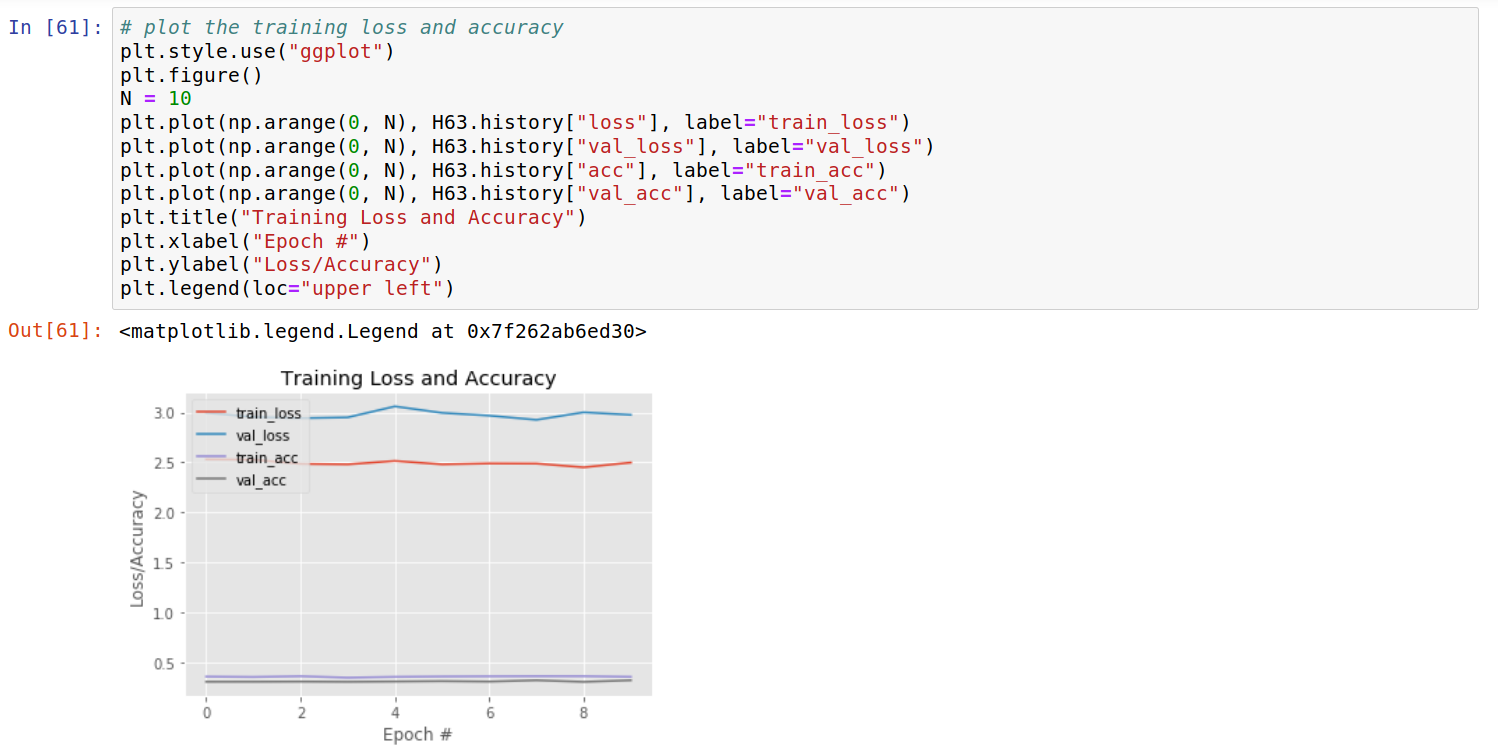
\includegraphics[width=\textwidth]{training_statistics.jpg}
%\caption[Bildbeschreibung]{\url{https://www.iosb.fraunhofer.de/servlet/is/78045/}}
\label{trainingStatistics}
\end{figure}
%In this section, the final model and any supporting qualities should be evaluated in detail. It should be clear how the final model was derived and why this model was chosen. In addition, some type of analysis should be used to validate the robustness of this model and its solution, such as manipulating the input data or environment to see how the model’s solution is affected (this is called sensitivity analysis). Questions to ask yourself when writing this section:
%
%Is the final model reasonable and aligning with solution expectations? Are the final parameters of the model appropriate?
%Has the final model been tested with various inputs to evaluate whether the model generalizes well to unseen data?
%Is the model robust enough for the problem? Do small perturbations (changes) in training data or the input space greatly affect the results?
%Can results found from the model be trusted?
\subsection*{Justification}
Unfortunately, we did not see other research results for logo classification with metric accuracy to compare these to our results.
However, given that the dataset had many logo classes with only few images, we think that we cannot expect a high overall accuracy. 
Still, we would like to reach an accuracy of at least 50 \% but we do not know which parameters of the different models from the previous sections, or which other CNN architectures could lead to a test accuracy higher than 40 \%.

On the other hand, our final model is robust and classifying small logos in larger images is not an easy task so our final result with a test accuracy of 30.91 \% is adequate.
%In this section, your model’s final solution and its results should be compared to the benchmark you established earlier in the project using some type of statistical analysis. You should also justify whether these results and the solution are significant enough to have solved the problem posed in the project. Questions to ask yourself when writing this section:
%
%Are the final results found stronger than the benchmark result reported earlier?
%Have you thoroughly analyzed and discussed the final solution?
%Is the final solution significant enough to have solved the problem?
\section{Conclusion}
%TODO
%(approx. 1-2 pages)

\subsection*{Free-Form Visualization}
In this subsection, we visualize some logo classification results on ten test images:
\begin{figure}[h!]

\includegraphics[width=\textwidth]{prediction_of_test_file_100.png}
\label{prediction1}
\end{figure}
\begin{figure}[h!]

\includegraphics[width=\textwidth]{prediction_of_test_file_101.png}
\label{prediction1}
\end{figure}
\begin{figure}[h!]

\includegraphics[width=\textwidth]{prediction_of_test_file_102.png}
\label{prediction1}
\end{figure}
\begin{figure}[h!]

\includegraphics[width=\textwidth]{prediction_of_test_file_103.png}
\label{prediction1}
\end{figure}
\begin{figure}[h!]

\includegraphics[width=\textwidth]{prediction_of_test_file_104.png}
\label{prediction1}
\end{figure}
\begin{figure}[h!]

\includegraphics[width=\textwidth]{prediction_of_test_file_105.png}
\label{prediction1}
\end{figure}\\
\begin{figure}[h!]

\includegraphics[width=\textwidth]{prediction_of_test_file_106.png}
\label{prediction1}
\end{figure}\\
\begin{figure}[h!]

\includegraphics[width=\textwidth]{prediction_of_test_file_107.png}
\label{prediction1}
\end{figure}\\
\begin{figure}[h!]

\includegraphics[width=\textwidth]{prediction_of_test_file_108.png}
\label{prediction1}
\end{figure}\\
\begin{figure}[h!]

\includegraphics[width=\textwidth]{prediction_of_test_file_109.png}
We note that some logo classes like Volkswagen seem to have a better accuracy than the others.
\label{prediction1}
\end{figure}
%In this section, you will need to provide some form of visualization that emphasizes an important quality about the project. It is much more free-form, but should reasonably support a significant result or characteristic about the problem that you want to discuss. Questions to ask yourself when writing this section:
%
%Have you visualized a relevant or important quality about the problem, dataset, input data, or results?
%Is the visualization thoroughly analyzed and discussed?
%If a plot is provided, are the axes, title, and datum clearly defined?
\subsection*{Reflection}
There were several obstacles when training a CNN to classify or detect logos.
At first, the local hardware was not sufficient so often the training process freezes or progresses only slowly. 
Also uploading the large dataset to Amazon Web Services or Google Cloud's bucket took very long.
Furthermore, when training a Faster R-CNN with Tensorflow's Object Detection API the error log was not sufficiently detailed to identify why there are no detections.

In addition to these technical limitations, further experience with CNNs is needed for adjusting the right parameters of the models. In the end, the very first two model architectures from \autoref{table:modelFromScratch} and \autoref{table:vgg_custom} already reach the best accuracy.

%In this section, you will summarize the entire end-to-end problem solution and discuss one or two particular aspects of the project you found interesting or difficult. You are expected to reflect on the project as a whole to show that you have a firm understanding of the entire process employed in your work. Questions to ask yourself when writing this section:
%
%Have you thoroughly summarized the entire process you used for this project?
%Were there any interesting aspects of the project?
%Were there any difficult aspects of the project?
%Does the final model and solution fit your expectations for the problem, and should it be used in a general setting to solve these types of problems?
\subsection*{Improvement}
As a first crucial improvement, one could use Scikit-learn's from MultiLabelBinarizer to label the images with potentially multiple logo classes from the corresponding XML files. This would lead to 821 classes instead of 109 but the logo images may be more accurately classified.
How to train a CNN with multiple label classification is described \href{https://www.pyimagesearch.com/2018/05/07/multi-label-classification-with-keras/}{here}.

The accuracy may also be improved by (additionaly / pre-)training with the ROI images of the Logos in the Wild dataset, which are generated by the Python script \path{create\_clean\_dataset.py}. We did not choose this option as our goal is to classify logos in any image. By construction, CNNs are relatively translation invariant so that our goal seems to be within reach.

Moreover, due to time limits we did not train our models very long. More epochs could also lead to higher accuracy and to choosing a different model than we did.

Similarly, there are many more reasonable parameter combinations to explore than we did in this short time. For instance, using different activation functions, various filter sizes or decreasing learning rates.

Last, of course training an object detection model may lead to better results like the one mentioned in our benchmark section. We do not know why we could not detect any logos with our Faster R-CNN but it makes sense to still further investigate this.
%In this section, you will need to provide discussion as to how one aspect of the implementation you designed could be improved. As an example, consider ways your implementation can be made more general, and what would need to be modified. You do not need to make this improvement, but the potential solutions resulting from these changes are considered and compared/contrasted to your current solution. Questions to ask yourself when writing this section:
%
%Are there further improvements that could be made on the algorithms or techniques you used in this project?
%Were there algorithms or techniques you researched that you did not know how to implement, but would consider using if you knew how?
%If you used your final solution as the new benchmark, do you think an even better solution exists?
%\subsection*{Before submitting, ask yourself...}
%
%Does the project report you’ve written follow a well-organized structure similar to that of the project template?
%Is each section (particularly Analysis and Methodology) written in a clear, concise and specific fashion? Are there any ambiguous terms or phrases that need clarification?
%Would the intended audience of your project be able to understand your analysis, methods, and results?
%Have you properly proof-read your project report to assure there are minimal grammatical and spelling mistakes?
%Are all the resources used for this project correctly cited and referenced?
%Is the code that implements your solution easily readable and properly commented?
%Does the code execute without error and produce results similar to those reported?



%\nocite{*}
\bibliography{capstone_project}
\bibliographystyle{alpha}
\end{document}
%
%     Your key must not be publicly viewable for SSH to work. Use this command if needed:
%
%    chmod 400 BasicE2.pem
%
%    Connect to your instance using its Public DNS:
%
%    ec2-3-120-244-179.eu-central-1.compute.amazonaws.com
%
%Example:
%
%ssh -i "BasicE2.pem" ec2-user@ec2-52-59-207-104.eu-central-1.compute.amazonaws.com -L 8889:127.0.0.1:8889

ssh -i "IrelandKey.pem" ubuntu@ec2-34-254-91-106.eu-west-1.compute.amazonaws.com -L 8889:127.0.0.1:8888

~/anaconda3/envs/tensorflow_p36/lib/python3.6/site-packages/tensorflow/models/research

rsync -av -progress -e "ssh -i IrelandKey.pem" /data/Machine_Learning/Machine_Learning_Engineer/capstone_project/LogosInTheWild-v2/data/voc_format ubuntu@ec2-34-241-125-193.eu-west-1.compute.amazonaws.com:~/capstone_project/LogosInTheWild-v2/data/voc_format


source activate tensorflow_p36

%    RUN sudo /etc/init.d/ssh start

%rsync -azvv -e ssh -i "IrelandKey.pem" /data/Machine_Learning/Machine_Learning_Engineer/capstone_project/LogosInTheWild-v2/data ec2-user@ec2-34-241-125-193.eu-west-1.compute.amazonaws.com:~/capstone_project/LogosInTheWild-v2/data 

rsync -azvv -e  ssh -i ~/.ssh/google_compute_engine /data/Machine_Learning/Machine_Learning_Engineer/capstone_project/LogosInTheWild-v2/data/ ajuschka@34.76.173.78:capstone_project/LogosInTheWild-v2/data



%scp -r -i "BasicE2.pem" /data/Machine_Learning/Machine_Learning_Engineer/capstone_project/LogosInTheWild-v2/ ec2-user@ec2-52-59-207-104.eu-central-1.compute.amazonaws.com :capstone_project/LogosInTheWild-v2/ 


scp -r ~/capstone_project/saved_keras_models/ ann-kristinlocalhost:/data/Machine_Learning/Machine_Learning_Engineer/capstone_project/saved_keras_models


%\begin{verbatim}
cd /mnt/c/ProgramData/anaconda3/envs/tensorflow/models/research
source ~/.bashrc
export PYTHONPATH=$PYTHONPATH:`pwd`:`pwd`/slim
PIPELINE_CONFIG_PATH=/mnt/c/environment/Machine_Learning/Machine_Learning_Engineer/capstone_project/LogosInTheWild-v2/models/model/faster_rcnn_inception_logos.config
MODEL_DIR=/mnt/c/environment/Machine_Learning/Machine_Learning_Engineer/capstone_project/LogosInTheWild-v2/models/model/
NUM_TRAIN_STEPS=20000
NUM_EVAL_STEPS=20
SAMPLE_1_OF_N_EVAL_EXAMPLES=1
TRAIN_DIR=/mnt/c/environment/Machine_Learning/Machine_Learning_Engineer/capstone_project/LogosInTheWild-v2/models/model/train
EVAL_DIR=/mnt/c/environment/Machine_Learning/Machine_Learning_Engineer/capstone_project/LogosInTheWild-v2/models/model/eval
python object_detection/model_main.py --pipeline_config_path=${PIPELINE_CONFIG_PATH} --model_dir=${MODEL_DIR} --num_train_steps=${NUM_TRAIN_STEPS}  
   --num_eval_steps=NUM_EVAL_STEPS --alsologtostderr

cd ~/anaconda3/envs/tensorflow_cpu/lib/python3.6/site-packages/tensorflow/models/research
export PYTHONPATH=$PYTHONPATH:`pwd`:`pwd`/slim
PIPELINE_CONFIG_PATH=/data/Machine_Learning/Machine_Learning_Engineer/capstone_project/LogosInTheWild-v2/models/model/faster_rcnn_inception_logos-locally-on-ubuntu.config
MODEL_DIR=/data/Machine_Learning/Machine_Learning_Engineer/capstone_project/LogosInTheWild-v2/models/model/
NUM_TRAIN_STEPS=20000
NUM_EVAL_STEPS=20000
SAMPLE_1_OF_N_EVAL_EXAMPLES=1508
TRAIN_DIR=/data/Machine_Learning/Machine_Learning_Engineer/capstone_project/LogosInTheWild-v2/models/model/train
EVAL_DIR=/data/Machine_Learning/Machine_Learning_Engineer/capstone_project/LogosInTheWild-v2/models/model/eval
python object_detection/model_main.py --pipeline_config_path=${PIPELINE_CONFIG_PATH} --model_dir=${MODEL_DIR} --num_train_steps=${NUM_TRAIN_STEPS} --num_eval_steps=${NUM_EVAL_STEPS} --alsologtostderr




python object_detection/legacy/train.py --logtostderr --train_dir=${TRAIN_DIR} --pipeline_config_path=${PIPELINE_CONFIG_PATH}  --alsologtostderr

 python object_detection/legacy/eval.py  --logtostderr   --pipeline_config_path=${PIPELINE_CONFIG_PATH} --checkpoint_dir=${MODEL_DIR}  --eval_dir=${EVAL_DIR}

YOUR_CLOUD_BUCKET=gs://logo-bucket-europe-west1//
PATH_TO_LOCAL_YAML_FILE=/data/Machine_Learning/Machine_Learning_Engineer/capstone_project/standard_gpu.yaml
GS_MODEL_DIR=logo-bucket-europe-west1/LogosInTheWild-v2/models/model
GS_TRAIN_DIR=logo-bucket-europe-west1/LogosInTheWild-v2/models/model/train
GS_EVAL_DIR=logo-bucket-europe-west1/LogosInTheWild-v2/models/model/eval
GS_PIPELINE_CONFIG_PATH=logo-bucket-europe-west1/LogosInTheWild-v2/models/model/faster_rcnn_inception_logos-europe-west1.config
# From tensorflow/models/research/
gcloud ai-platform jobs submit training object_detection_`date +%m_%d_%Y_%H_%M_%S` --runtime-version 1.13 --job-dir=gs://${GS_MODEL_DIR} --packages dist/object_detection-0.1.tar.gz,slim/dist/slim-0.1.tar.gz,/tmp/pycocotools/pycocotools-2.0.tar.gz --module-name object_detection.model_main --region europe-west1 --config ${PATH_TO_LOCAL_YAML_FILE} -- --model_dir=gs://${GS_MODEL_DIR} --pipeline_config_path=gs://${GS_PIPELINE_CONFIG_PATH} 


gcloud ml-engine jobs submit training object_detection_`date +%m_%d_%Y_%H_%M_%S` --runtime-version 1.13 --job-dir=gs://${GS_TRAIN_DIR} --packages dist/object_detection-0.1.tar.gz,slim/dist/slim-0.1.tar.gz,/tmp/pycocotools/pycocotools-2.0.tar.gz --module-name object_detection.legacy.train --region europe-west1 --config ${PATH_TO_LOCAL_YAML_FILE} -- --train_dir=gs://${GS_TRAIN_DIR} --pipeline_config_path=gs://${GS_PIPELINE_CONFIG_PATH}

gcloud ml-engine jobs submit training object_detection_`date +%m_%d_%Y_%H_%M_%S` --runtime-version 1.13 --job-dir=gs://${GS_EVAL_DIR} --packages dist/object_detection-0.1.tar.gz,slim/dist/slim-0.1.tar.gz,/tmp/pycocotools/pycocotools-2.0.tar.gz --module-name object_detection.legacy.train --region europe-west1 --config ${PATH_TO_LOCAL_YAML_FILE} -- --eval_dir=gs://${GS_EVAL_DIR} --train_dir=gs://${GS_TRAIN_DIR} --pipeline_config_path=gs://${GS_PIPELINE_CONFIG_PATH}


%train
  $ gcloud ml-engine jobs describe object_detection_04_29_2019_20_38_31

or continue streaming the logs with the command

  $ gcloud ml-engine jobs stream-logs object_detection_04_29_2019_20_38_31

 


sudo apt-get install ssh
sudo /etc/init.d/ssh start

tensorboard --logdir=${MODEL_DIR}
%\end{verbatim}



### Setting up Google Bucket Storage (instead of creating TFRecord files in Step 10)

-- Install [gsutil](https://cloud.google.com/storage/docs/gsutil_install#sdk-install)

-- Run gcloud init and gcloud auth application-default login

-- Download dataset from Google bucket 
``` bash
# From Logo Capstone Project directory
gsutil cp -r gs://logo-bucket-europe-west1 .
```

gsutil -m cp -r gs://logo-bucket-europe-west1/LogosInTheWild-v2/data capstone_project/

-- YOUR_CLOUD_BUCKET=gs://logo-bucket-europe-west1//
tensorboard --logdir=${YOUR_CLOUD_BUCKET}

%gcloud compute ssh gpu-deep-learner --zone europe-west1-d
ann-kristin@gpu-deep-learner:~$ exit
logout
Connection to 34.76.173.78 closed.

ssh -i .ssh/google_compute_engine ajuschka@34.76.173.78 -L 8899:localhost:8888


tf.logging.set_verbosity(tf.logging.INFO)